\documentclass{llncs}
\usepackage[T1]{fontenc}
\usepackage[swedish]{babel}
\begin{document}

\title{PHP Framework Performance for Web Development}
\titlerunning{PHP Framework Performance}  
% abbreviated title (for running head)
%                                     also used for the TOC unless
%                                     \toctitle is used
%
\author{H�kan Nyl�n}
%
\authorrunning{H�kan Nyl�n}   % abbreviated author list (for running head)
%
%%%% list of authors for the TOC (use if author list has to be modified)
\tocauthor{H�kan Nyl�n}
%
\institute{Blekinge Institute of Technology, Karlskrona, Sweden,\\
\email{hakan@dun.se}}

\date{21 March, 2012}

\maketitle
% A category with the (minimum) three required fields
%\category{H.4}{Information Systems Applications}{Miscellaneous}
%A category including the fourth, optional field follows...
%\category{D.2.8}{Software Engineering}{Metrics}[complexity measures, performance measures]

%\terms{Theory}
\section{Intro}
PHP Framework is a new thinking, making it faster to build a website. You can have a good structure and found things faster, You can add new features more quickly. But, does it have good performance? We talk all the time about fast development, but performance is under the hood very important. People seems to forget the importance, except from few systems and new ideas, like CDN\footnote{CDN is Content Delivery Network, a network of servers, where static data for websites and more can be stored, a CDN is spread all over the world, making the request faster.} makes it faster wherever you are in the world. But how is the performance in PHP framework? is it as fast as how fast it is to develop in it?

\section{The Background}
Evaluation is all about the performance. Performance in this paper is about load\footnote{loads means how long a request take, in milliseconds.}, but it can be hardware, network and so on. Evaluation in general is how you can test the performance and in which way. This is very important in the choice of products nowadays.

\subsection{PHP Framework}
PHP is a server-side programming language famous to make it simple to develop in agile methods in web development. The Frameworks are built on MVC-thinking with addons, like form-helpers and database-controller, in various languages, like PHP, which we use in this paper. Frameworks are built to make it even more faster to develop a website. The biggest PHP Frameworks with MVC-thinking are CodeIgniter\cite{MVC:codeigniter} and CakePHP\cite{MVC:cakephp}.

\subsection{MVC}
Model View Controller is a structure-think to have 3 different types of classes, typing of what they will do. \cite{MVC:phpTeam} Model will handle data, like database. View is the one that handle how the data should be shown. Controller is the middle, getting data from model and fixing the data  and sending it on to the View. This paper will be about testing the performance of CodeIgniter \cite{MVC:codeigniter} and CakePHP \cite{MVC:cakephp}, these are MVC frameworks in PHP.

\subsection{Client-side}
Client-side is meaning, in this thesis, the browser and the scripts and other rendering happening by the visitor on the site. This does have a big impact in the in performance for a server. \cite{performance:Understanding} If using many images, the browser first loads the page and then send request for the image and scripts on the page, adding more load to the server, because of more request which load the network for the server. \cite{performance:dynweb}

\subsection{Server-side}
Server-side is the server, of course. Here can the network, CPU and RAM be a impact in the performance for the visitor of the site. \cite{performance:dynweb} Often is the network that is stopping more load to the server, because the optimized server program such as Apache don\'{}t use so much of the CPU and RAM, making  the CPU and RAM the less problem. Of course can that be the issue, but not so often.

\subsection{Performance}
What performance can be different, in this paper I mean it as fast request, so network is very important. It can also have big impact how the servers is, Like a big server park in a datacenter. But I don\\'{}{}t have time or money to try that. That\\'{}{}s why I will only test this on cloud with one server and see how the framework is changing the ms of a request.

\section{Research}
\subsection{Research Questions}
\begin{description}
  \item[RQ1:] What web performance evaluations exist and how were they performed?
  \item[RQ2:] What factors impact web performance?
  \item[RQ3:] To what extent are open source php frameworks evaluated?
  \item[RQ4:] What performance are different between most commonly used open source php frameworks and how can it be evaluated?
\end{description}
I searched more or less on different types of strings like ``web development evaluation\'{}\'{} and ``Web development performance\'{}\'{}. I found 300 papers and 8 relevant because the others was talking about the evaluation in general, not about performance in web development. 


\subsection{Research Methodology}
  \begin{tabular}{ l  r }
     
    Research Question & Methodology \\ 
    \hline
    RQ1 & Literature \\ 
    RQ2 & Literature \\
    RQ3 & Literature \\
    RQ4 & Data from RQ1, RQ2 and RQ3 to design experiment \\
  \end{tabular}
\subsection{Literature Survey}
The literature is found in different stages. And I used this Sources.
\begin{description}
  \item Google Scholar
  \item IEEE
  \item Google
  \item 
\end{description}

This strings was used, seeing in Figure \ref{fig:literaturesearchstrings}.
\begin{figure}[htbp]
\centering
\begin{tabular}{ p{6cm}}
  Strings\\
  \hline
  Web development Evaluation \\
  Web development Performance \\
  PHP Framework evaluation \\
  PHP Framework performance \\
  PHP Evaluation \\
  PHP Performance \\
  Website Performance \\
  Website evaluation \\
\end{tabular}
\caption{The strings for searching literature}
\label{fig:literaturesearchstrings}
\end{figure}

The selection wasn\'{}t so hard, I was looking for some data that was doing something with evaluation in this area, and it is a few. I was looking for good howto, how they made the research to find out the information in the data. Often it was over 300 results in the search, but only 1-3 relevant pages, in every string, and the papers was often in many of the strings.

\section{Literature review}
\subsection{The Approach}
I searched by the string presented in Figure \ref{fig:literaturesearchstrings}, found some hundreds of papers. This comes to the approach that I tried to found some with text such as impact in performance or was something about performance in PHP, because of the lack of papers in this area so was it hard to even find this. I took all I could found in this area, that have something that could be used for the questions to be answered such as impact in evaluation tests, php frameworks, different evalution types and hows. I have big experience in php development so the php framework was easy to find the little papers I could found. The rest was must in how my interest in performance and knowing to found something about impact that was the biggest.
\subsection{The Papers}
The information what the papers is and what they have in common.
\subsubsection{PHP Team Development}
is about how the MVC idea and technique make a difference in the development. This is a book about how the development in PHP is and what they do, as MVC is a big part of it. This book is from 2009.

\subsubsection{Analysis of model-based mvc framework for php development CodeIgniter}
is analysing how the mvc based framework Codeigniter is doing in the development in performance and in userability for developers. this is a analysing paper from May 2009, it has kinda much in common with PHP Team Development, the book which have a chapter about MVC. 

\subsubsection{Ec2 faq: What is a ec2 compute unit}
shows what EC2 is about and what a compute unit is, to how something to reference to for the server specification in the tests. This is a website FAQ, which was last visited april 2012.

\subsubsection{Understanding web performance}
presents how performance can be used and it\'{}s importance in the web business, it also bring up how performance can be tested and what can be a impact for the tests. It\'{}s a paper presented in a Business Communication Review October 2001. 

\subsubsection{A performance comparison of dynamic web technologies}
describe the different impact in performance when they do a comparison in different performance types and how that can be done. Presented in ACM Sigmetrics December 2003.

\subsubsection{Web-based ide to create model and controller components for mvc-based web applications on cakephp}
writes how the CakePHP is build and how to code in it and talk a little about how MVC is about. A normal paper from December 2010. Has much in common with the other MVC framework Codeigniter and the book PHP Team Development.


\newpage
\section{Literature Results}

\subsection{RQ1: What web performance evaluation exist and how were they performed?}
Evaluation in web is mostly done in loads and counted in ms, but also in how to optimize the page itself to minimize request to server, like less pictures, or move them to another server. This can be seen in Figure \ref{fig:rq1evaluation}.
\begin{figure}[htbp]
\centering
\begin{tabular}{ p{4cm} p{3cm} p{2cm} }
  Evaluation topic & How & year\\
  \hline
  	requests/ms & Experiment & 2001\cite{performance:Understanding}\cite{performance:dynweb}\\
  	server/cpu & Experiment & 2003 \cite{performance:dynweb} \\
  	on-page optimization & Experiment & 2003\cite{performance:dynweb}\\
\end{tabular}
\caption{Different types of evaluation of a web performance}
\label{fig:rq1evaluation}
\end{figure}

{\bf request/ms} is the most used to evaluate performance of web applications. i got two different pappers talking about two different things, \emph{Understanding Performance} adds this comment:
\begin{quote}
Sure, speed matters, but it\'{}s not a one-dimensional problem. And, despite what you\'{}ve heard, just adding more bandwidth doesn\'{}t always make things go faster. \cite{performance:Understanding}
\end{quote}
High requests needs good cpu and network, but to understand \emph{Understanding Performance} speed matters but not always the only problem. \emph{A Performance Comparison of Dynamic Web Technologies} talks about something how they do the tests with requests in ms:
\begin{quote}
Consideration of over- load behaviour may be just as important as the peak request rate when Web site administrators are choosing dynamic Web content generation technologies. \cite{performance:dynweb} 
\end{quote}
They saw a important to consider how to choose technologies using dynamic web content, because of different peak of request in how big the request was. They also show how good it can be to evaluate how the performance is by using requests per milliseconds, or seconds.

{\bf server/cpu} is important when the server need to handle many request in the same time. \emph{A Performance Comparison of Dynamic Web Technologies} tells that: 
\begin{quote}
Once the servers become overloaded, the CPU utilization of Apache 2.0.45 is lower than that of Apache 1.3.27. Under overload, Apache 2.0.45 is unable to accept TCP connections (and hence re- quests) as quickly as Apache 1.3.27. \cite{performance:dynweb}
\end{quote}
Making it important for cpu to work, but that\'{}s doesn\'{}t mean that Apache itself make the CPU overload, it can be the network the cpu need to handle.

{\bf On-page optimization} is about how to create less request to the server by removing or group images to one, because browsers loads the html first and then sending more request to get the images. This does also have a thing with the size of the images as well, Bigger images make it longer time to download it. \emph{A Performance Comparison of Dynamic Web Technologies} is testing with static content \cite{performance:dynweb} that can be images or normal html files. Showing it goes faster then dynamic content, but it is a request.

\subsection{RQ2: What factors impact web performance?}
There are things that can be a impact of the performance while testing. The impact i could see is listed in figure \ref{fig:rq2evaluation}.
\begin{figure}[htbp]
\centering
\begin{tabular}{ p{2cm} p{3cm} p{7cm} }
  Factor & How it impact & comment\\
  \hline
  	Server & network, cpu, ram & This can be fixed with a big server or a datacenter, something I can\'{}t test here.\\
  	\hline
  	Network & speed & if I will do a request/ms load simulation, my network can be maximized without the server being touched to the performance limit I want.\\
  	\hline
  	Wrong config & slowness, bad performance & wrong config on the server can make it extra slow, but i will not think about that. I will only use the default settings. This is not a optimization paper.
\end{tabular}
\caption{Different types of evaluation of a web performance}
\label{fig:rq2evaluation}
\end{figure}

{\bf The server} can have big impact of the performance because the cpu and RAM can be to less to handle the big amount of request tested. Small CPU and RAM can make it to overload in power and deny new request. Making it impossible to connect when that amount of request is full.

{\bf The Network} is not very important but the network should be stabile and workable for the amount of request sending to the server. Normal speed would be at least 10mbit down and 10mbit up to send and receive in good speed. The only problem with the network in my home is the stability, making it hard to trust the speed, making the ms higher then it should be. I can have 100mbit up and 100mbit down, but only getting 34 mbit of both because we share the internet connection in the whole house, which I just live in apartment in.

{\bf Wrong config} is almost the thing that can be spooky and many people don\'{}t know that it can be a default config or a wrong setup config that make the server to overload or not accept requests. The tests will use defaults just to make it so not touchable as possible, because of how many people that actually is using the defaults in the configs.

\subsection{RQ3: To what extent are open source php frameworks evaluated?}
It was nothing about how performance in php framework what I could found, this is one of the things why I want to experiment and do this. I see a big area in performance in php framework not covered.

\section{Experiment Design} 

\subsection{Investigated Question}
Which of the following php framework provide better performance measured in terms at: page speed in ms.

\subsection{Experiment artifacts and variables}


\subsubsection{Controlled Variables}
the following variables are controlled
\begin{figure}[htbp]
\centering
\begin{tabular}{ p{3cm} p{7cm} }
  	Variable & Description\\
  	\hline
  	Request size & constant\\
  	Server & see figure \ref{fig:serverSpecification}\\
  	Framework & Compatible API, look at figure \ref{fig:classes} for info about the classes to use.\\
  	Response size & constant
\end{tabular}
\caption{Controlled variables in Experiment}
\label{fig:controlledvariables}
\end{figure}

The tests is as you can see in the list below, all 3 tests will be run for database and without database, for each framework. Making it 6 tests total for a framework, with and without database.
\begin{description}
  \item[Test 1] 5, 20,000
\begin{figure}[htbp]
\centering
\begin{tabular}{l l l l l l}
&\multicolumn{2}{l}{Codeigniter}&\multicolumn{2}{l}{CakePHP}\\
\cline{2-5}
 &Concurrency&Requests&Concurrency&Requests\\
 Test 1 & 5 & 20,000 & 5 & 20,000 & with database\\
 Test 2 & 5 & 20,000 & 5 & 20,000 & with database\\
 Test 3 & 5 & 20,000 & 5 & 20,000 & with database\\
 \hline
 Test 1 & 5 & 20,000 & 5 & 20,000 & withOUT database\\
 Test 2 & 5 & 20,000 & 5 & 20,000 & withOUT database\\
 Test 3 & 5 & 20,000 & 5 & 20,000 & withOUT database\\
\end{tabular}
\caption{How the tests will make for the frameworks.}
\label{fig:testsforframework}
\end{figure}
I choice 5 for the concurrency level, meaning to send 5 request each time. This to help to count the response time more exactly. You can see how the tests will be done in figure \ref{fig:testsforframework}.

The total amount of request of 20,000 is to get okay amount of request to get average time from, not too much and not too less. It doesn\'{}t need to be much more because the average will be the same $\pm$ 2 ms. That make it not necessary to have more. But i took as much as 20,000 because it make it more sure to be right numbers in the results.

A good thing to know is how the server will be setup, here is the table of the specification of the server I will use for the experiment, on the Amazon cloud.
\begin{figure}[htbp]
\centering
\begin{tabular}{ p{4cm}	 p{4cm} }
  System & Version/size \\
  \hline
  OS & Ubuntu 10.04 \\
  Apache & 2.2.14 \\
  MySQL & 5.4 \\
  PHP & 5.3.2 \\
  CPU & 1 EC2 Compute Unit\footnotemark[3] \\
  RAM & 1.7 GB \\
  HDD & 160 GB \\
  bits & 64 bit
\end{tabular}
\caption{The server specification where the test will be done on.}
\label{fig:serverSpecification}
\end{figure}
This is how the Framework classes will be used in the experiment.
\footnotetext[3]{One EC2 Compute Unit provides the equivalent CPU capacity of a 1.0-1.2 GHz 2007 Opteron or 2007 Xeon processor. \cite{EC2:Amazon}}
\begin{figure}[htbp]
\centering
\begin{tabular}{ p{3cm} p{3cm} p{3cm} }
  Type & Codeigniter class & CakePHP class\\
  \hline
  	Controller & CI\_{}Controller & AppController\\
  	Model & CI\textunderscore{}Model & AppModel\\
	Database & database & database \\
	Form helper & form & Form\\
\end{tabular}
\caption{The different classes to use in the frameworks while coding a blog.}
\label{fig:classes}
\end{figure}
\subsubsection{Manipulated variables}
Server load measured in terms of amount of request.

Manipulated variables
\begin{description}
  \item[Response Type] HTML without database, HTML with database
\end{description}

Response Type is the only thing i will change. It is the support of the database that will be removed or added, making it possible to see the difference in performance for the core of the framework and for just the database controller.

\subsubsection{Experiment Artifact}
\begin{description}
  \item[blog] the blog will have normal features, or more likely very simple. It will have a normal list with pagination on the startpage, every post will have its own page.
  \item[apache benchmark] will use Apaches own benchmark to simulate server load. 
  \item[Environment] the server is mostly already set, see figure \ref{fig:serverSpecification}.
\end{description}

{\bf Blog} is first a simple blog, with posts list on the startpage and with a own page for single post. The most important with the blog is the index page in this experiment because it is there i will send the requests. So i focused to make a decent list of posts with title, body and created date. Both frameworks use same database making it simple and less chance for the database to make a bad impact in the performance.

{\bf Apache benchmark} is picked because it seem it was the most workable tool to test performance for the web. All tools for performance for a web application is doing it it almost the same, it is same idea, to send a amount of request to the server and count how long it took to get a response back. Apache benchmark is the one that is been in while and has a reputation to do fair tests.

\section{Experiment}
\subsection{How it was made}

I used Apache benchmark to send request on 20,000 request on a currency on 5 request per time to a server. I made the test with a database on the night randomly picked which framework to test. The tests without database was made on the day, making it more sense why the ms is higher on the tests there, it is more traffic on the internet on the day.

I used ab -wn 20000 -c 5 http://11.11.11.11\footnote[4]{the ip is typed as 11.11.11.11 to make it clear that the server is not up no more}/framework to send the load request, randomly from my own computer to the test server, on the Amazon cloud on Ireland.

The variables controlled was response size, amount of request and currency of requests. see the data for the variables in figure \ref{fig:thedatafortests}.
\begin{figure}[htbp]
\centering
\begin{tabular}{ p{2cm} p{2,5cm}  p{2,5cm}  p{2,5cm}  p{2,5cm} }
  Variable & Codeigniter db\footnotemark[5] & Codeigniter & cakephp db\footnotemark[5] & cakephp \\
  \hline
  ResponseSize\footnotemark[6] & 6440000 bytes & 6440000 bytes & 6360000 bytes & 6360000 bytes \\
  Requests & 20,000 & 20,000 & 20,000 & 20,000 \\
  Currency & 5 & 5 & 5 & 5 \\
\end{tabular}
\caption{The tests with database average request/connection times in ms.}
\label{fig:thedatafortests}
\end{figure}
\footnotetext[5]{with db i mean database, so it is the framework with the database, the database was used with models for posts, without db it was just plain html in view with controller used.}
\footnotetext[6]{ResponseSize is total bytes of html sent from the server in one test, on every interval.}
\newpage
\subsection{The results}
The experiment was made randomly on a night in different times, picked randomly. there was 3 tests on each framework on 20,000 request total, 5 request per time when sending to the server.

The result can you see in figure \ref{fig:experimentwithdb}. It was almost same results on both, but a small gap between the two framework on just a few Millie seconds, to be exact, it was a gap on 5,34 ms in a average.
\begin{figure}[h]
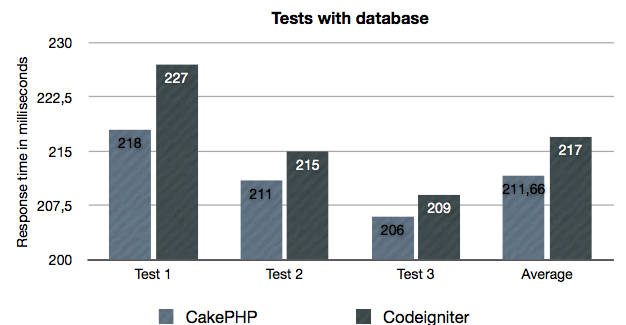
\includegraphics[scale=0.55]{charts-tests-database.png}
\caption{The tests with database average request/connection times in ms.}
\label{fig:experimentwithdb}
\end{figure}
\newpage
This was with database, with show that if we will focus to the ms total average, is CakePHP faster. This need to be tested without a database too, You can see the result in figure \ref{fig:experimentwithoutdb}.
\begin{figure}[h]
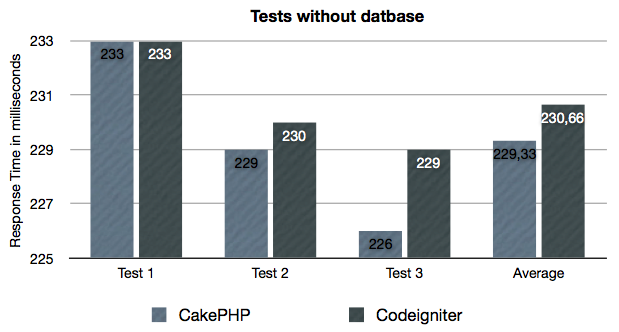
\includegraphics[scale=0.55]{charts-tests.png}
\caption{The tests without database average request/connection times in ms.}
\label{fig:experimentwithoutdb}
\end{figure}

The test without database shows that they are almost equally fast. only 1,3 ms gap between them, CakePHP was faster here too, showing CakePHP has faster structure in it\'{}s core.

\subsection{Data analysis and discuss}
This was good to  see how the different the performance is between the framework. This is also a very good way to evaluate the performance on any web service or application, the load of request can show how fast the request can be handled by the framework and show the fastness of it.

The biggest difference of the performance was when using a database, The difference was {\bf 5,34 ms}. it sounds little but in big sites just few ms does matter. The difference when using no database, only controller and view was kinda different, there was the difference {\bf 1,3 ms}. very little. and if we bring the size in the thought, the gap is even lesser. Maybe is Codeigniter faster, if they was in same size? That can be true. I used the default template in CakePHP and Codeigniter making it different in size, and could make a difference in the performance of the tests and request.

{\bf The difference in milliseconds} is so small without database because the frameworks seems to have good structure in their core of controllers and support for views, which we used in the tests without database for both framework. The difference in milliseconds for the tests with a database is bigger, 5.34 ms. Smaller then a thought but it is a difference. making it noticeable when having a database and the PHP framework on a big website with many visitors. Creating a big queue of requests, making the small difference bigger, 5.34 ms can feel like the double, 10,68 ms or more. That\'{}s why a small difference can be important.

A thing to think about is the size difference, which was around {\bf 80,000 bytes}, for both the test with and without the database. This can make gap between the framework understandable with db, but without the db was the tests very close to each others. If the size was the same, Codeigniter could be faster. 

The difference in the size is because i used the default in CakePHP and Codeigniter, CakePHP has more style and a usable template as default for the application, Codeigniter don\'{}t have it making it confused of the bigger size of the response. But the size is not a problem because i choose to use the default of each framework, making the difference in the size.

I see this as a no problem, i used the default tools in both framework to make a very simple blog webpage. The size should in other word be different, it would be weird if it wasn\'{}t. But i thought that the size can make a difference is of course in the mind. It is request time in ms, and it does have a very big impact by the size.

I would love to see {\bf future work} on different sizes for the PHP framework, which tests how the size does matter of the performance, with same size of both.

\section{Conclusion}
The frameworks performance has big difference, but mostly just if in used of database, the classes fro using database can in other words be more effective. CakePHP was fastest in both tests, with and without a database. But the size was different on 80,000 bytes. This could be something that could make CakePHP a winner. But my conclusion is that i used default template, very simple html page. So it doesn\'{}t have a big impact.

The fastest framework, according to the data is CakePHP, with just 1,3 ms without database and with 5,34 ms with database. This is something that is a big impact in the PHP performance and it can be fixed in newer versions. 

The experiment shows that the evaluation can be done it milliseconds for websites and web applications. 
With this data is the difference of evaluation between PHP framework not big at all, but it is a difference, even if it is a small one. 

The relevance and contribution of this paper is big because of the lack of papers and experiment made on PHP Frameworks. This is one of a new area of technology to test in performance.

Let the war begin between the php frameworks in performance.
\newpage
\renewcommand\refname{References}
\bibliographystyle{abbrv}
\bibliography{sigproc} 

\end{document}
